
%-----------------------------------------------------------------------------%
\chapter{\babSatu}
%-----------------------------------------------------------------------------%
Bab ini menjelaskan latar belakang, permasalahan, tujuan dan ruang lingkup 
penelitian, serta sistematika penulisan tugas akhir penelitian 

%-----------------------------------------------------------------------------%
\section{Latar Belakang}
%-----------------------------------------------------------------------------%
Kemampuan komputasi komputer berkembang seiring berjalannya waktu. Komputer mula - mula merupakan alat untuk melakukan operasi matematika semata. Namun seiring berkembangnya kebutuhan manusia, komputer tidak hanya melakukan operasi matematika semata. Komputer dipergunakan diberbagai bidang pekerjaan manusia, seperti industri kreatif perancangan \textit{design},\textit{game},pembuatan film, studio musik, pengolahan dokumen, maupun fungsi utama semula komputer, kemampuan komputasi untuk penelitian dalam bidang pendidikan.
\newline
\hspace{1.5cm}Pemanfaatan komputer dalam bidang penelitian mencakup berbagai hal. Dimulai dari penyimpanan data - data mentah yang nanti akan diolah dalam suatu proses aritmatika maupun data - data hasil pengolahan yang akan dilanjutkan dalam penelitian selanjutnya atau dibagikan dengan rekan sepenelitian. Beberapa bidang penelitian melakukan pengolahan data yang memerlukan kemampuan komputasi yang besar. Salah satunya adalah \textit{drug discovery}. Kemampuan ini dapat diperoleh dengan menggunakan \textit{supercomputer}. Terlepas keuntungan yang diperoleh dari pemanfaatan \textit{supercomputer}, terdapat kendala utama bagi para peneliti khususnya di negara berkembang. Kendala tersebut adalah besarnya dana yang harus dialokasikan dalam pengadaan \textit{supercomputer}. Tidak hanya itu saja, dengan semakin besarnya proses komputasi yang ada, maka semakin besar asumsi daya dibutuhkan oleh \textit{supercomputer}. Diperlukan pengetahuan khusus dalam merawat \textit{supercomputer}, sehingga para peneliti tidak hanya fokus dengan penelitiannya, namun dengan pengoperasian dan perawatan \textit{supercomputer} tersebut. Dan yang terakhir adalah alokasi tempat yang strategis untuk meletakan \textit{supercomputer} tersebut ditempat yang aman sehingga \textit{supercomputer} tidak mudah rusak dan data - data penelitian terjamin keamanannya 
\\
Salah satu alternatif yang dapat digunakan untuk menggantikan \textit{supercomputer} adalah pemanfaatan teknologi \textit{cloud computing}. Dengan ketiga sifat \textit{cloud computing} yaitu virtualisasi, distribusi, dan kemudahan dalam pengembangan dapat menutupi kekurangan \textit{supercoomputer}. Kemampuan virtualisasi dalam \textit{cloud computing} membuat seolah olah kita dapat mengoperasikan lebih dari 1 komputer walaupun hanya terdapat 1 \textit{server}. Selain itu peneliti tidak perlu mengetahui secara detail bagaimana teknologi ini bekerja dan perawatannya sehingga mereka dapat berfokus dengan penelitian yang sedang dikerjakan.
\begin{figure}
	\centering
	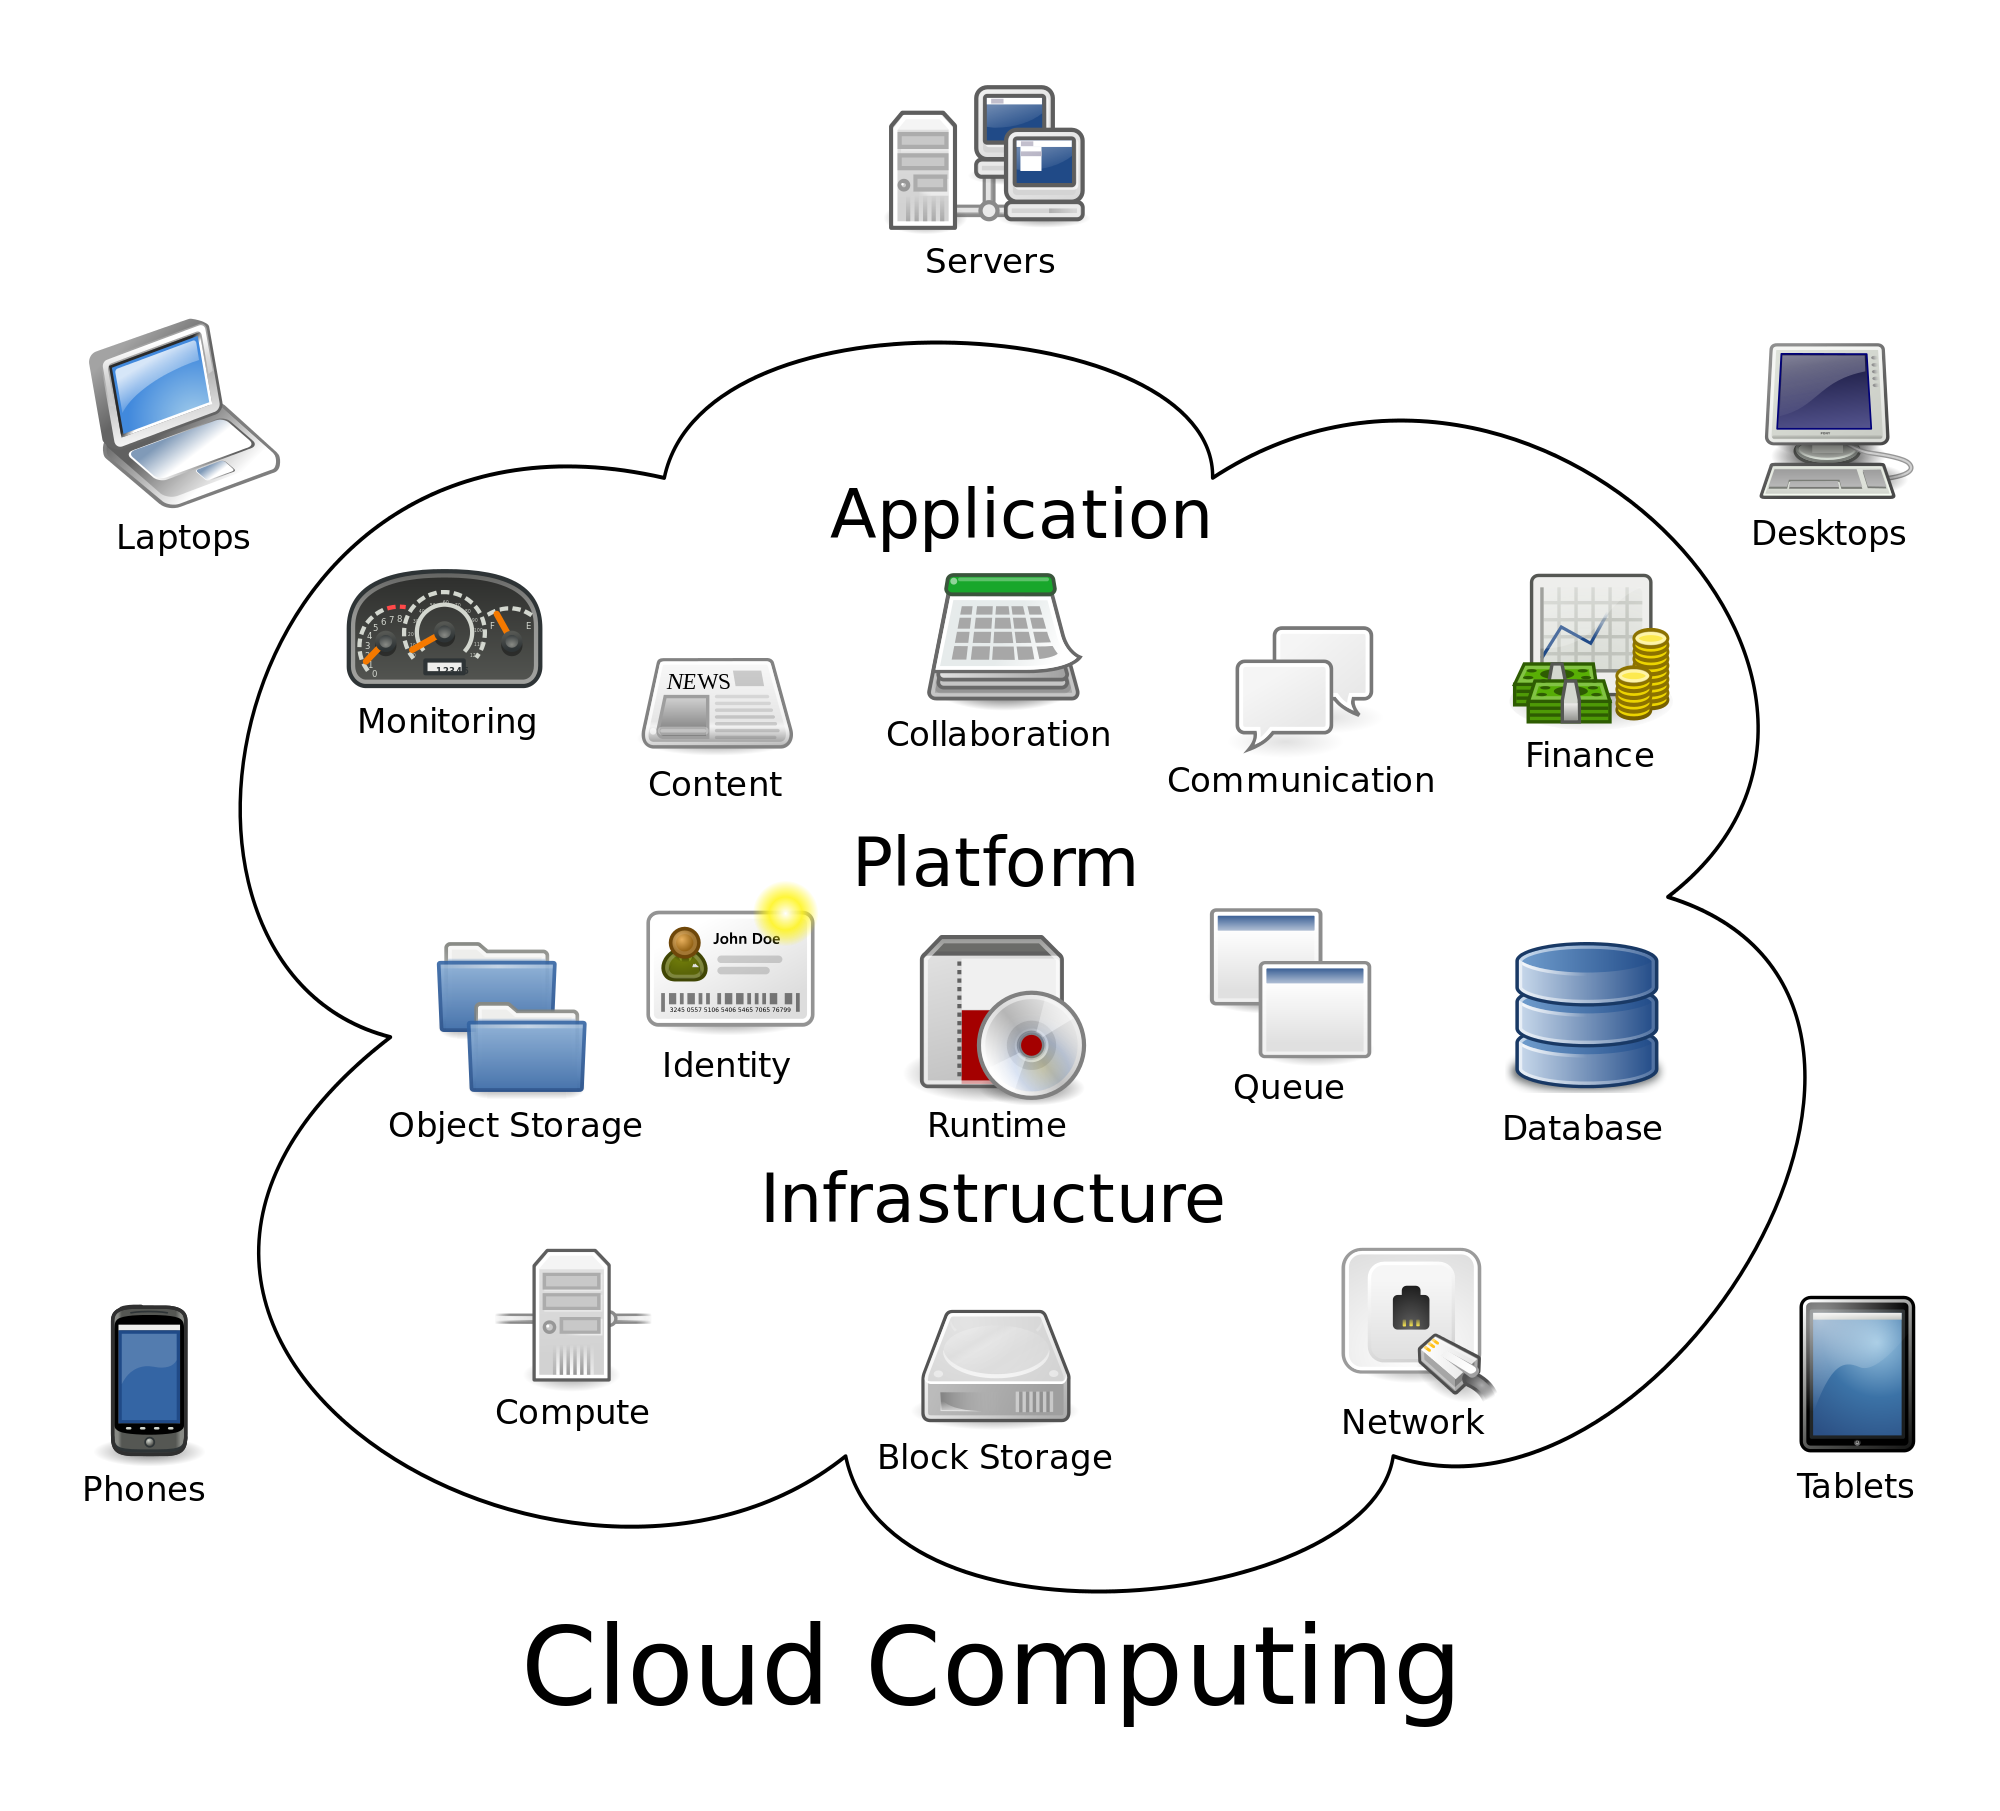
\includegraphics[scale=0.1]{cloud_computing.png}
	\caption{Ilustrasi Cloud Computing}
\end{figure}
Permasalahan yang muncul ketika memanfaatkan \textit{cloud computing} adalah bagaimana kita dapat mendapatkan kemampuan komputasi yang serupa dengan \textit{supercomputer}. Dengan sifat virtualisasi \textit{cloud computing} , kita dapat menjalankan banyak \textit{operating system} dalam 1 \textit{server}. Namun perlu upaya untuk mengoptimisasi virtualisas tersebut sehingga dapat memaksimalkan jumlah \textit{operating system } yang dapat berjalan dalam sebuah server. Salah satu aplikasi yang memiliki keunggulan dalam virtualisasi adalah Docker
\begin{figure}
	\centering
	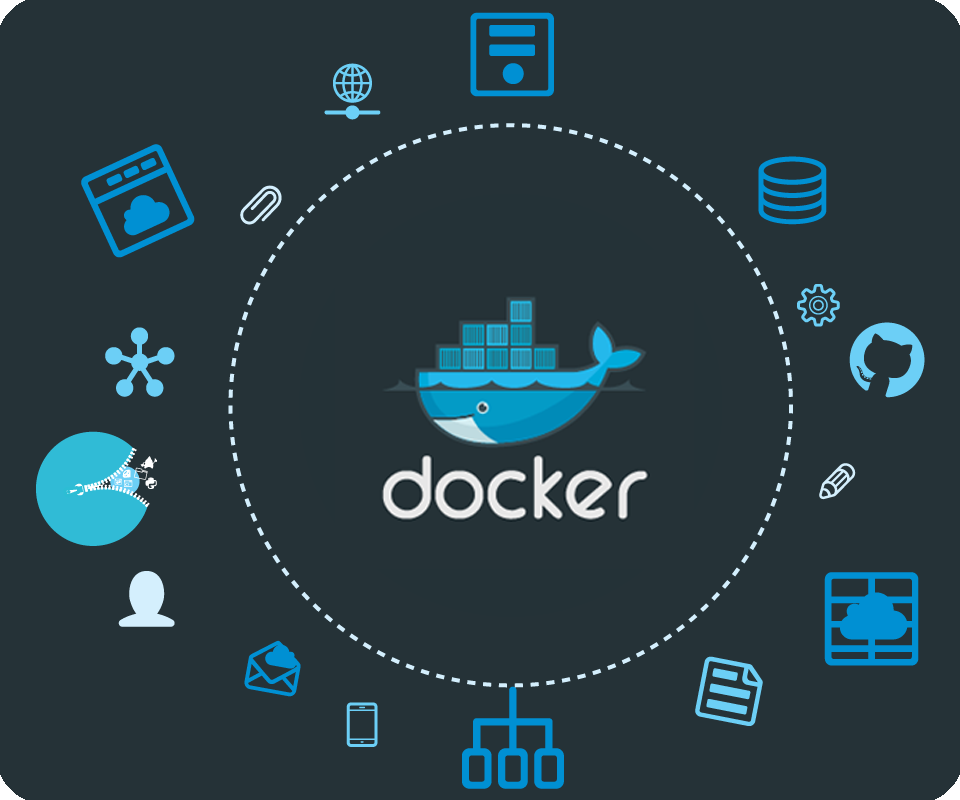
\includegraphics{docker.png}
	\caption{Docker}
\end{figure}

 

%-----------------------------------------------------------------------------%
\section{Permasalahan}
%-----------------------------------------------------------------------------%
%-----------------------------------------------------------------------------%
\subsection{Definisi Permasalahan}
%-----------------------------------------------------------------------------%
Berdasarkan latar belakang yang telah dijelaskan, penulis berusaha untuk menganalisis apakah pemanfaatan teknologi \textit{cloud computing}dengan menggunakan \textit{platform} Docker untuk virtualisasi komputer dapat diajukan sebagai solusi alternatif dari \textit{supercomputer} dan apakah performa yang diberikan oleh Docker tidak berbeda jauh dengan \textit{grid computing}. Untuk itu, penulis akan mencoba \textit{virtual screening} yang terdapat dalam \textit{drug discovery} dengan menggunakan aplikasi Autodock dan Autodock Vina yang terinstall pada Docker.

%-----------------------------------------------------------------------------%
\subsection{Batasan Permasalahan}
%-----------------------------------------------------------------------------%
Pada penelitian ini, penulis lebih berfokus kepada performa Docker dalam menjalankan aplikasi Autodock dan Autodock Vina untuk \textit{virtual screening}. Penulis tidak akan membahas segi \textit{virtual screening} dikarenakan keterbatasan pengetahuan yang dimiliki. 

%-----------------------------------------------------------------------------%
\section{Tujuan}
%-----------------------------------------------------------------------------%
Penelitian ini secara umum bertujuan untuk mengenalkan pemanfaatan \textit{platform} Docker dalam virtualisasi komputer yang digabungkan dengan teknologi \textit{cloud computing} untuk menghasilkan performa komputasi dengan harga terjangkau dibandingkan dengan pengadaan \textit{supercomputer} maupun \textit{grid computing}.


%-----------------------------------------------------------------------------%
\section{Posisi Penelitian}
%-----------------------------------------------------------------------------%
Penelitian ini mencari alternatif lain dari \textit{supercomputer} dengan memanfaatkan teknologi \textit{cloud computing}. Hasil dari penelitian ini akan dibandingkan dengan hasil penelitian serupa yang telah dikerjakan oleh Bapak Muhammad Hafizhuddin Hilman, S.Kom., M.Kom.

%-----------------------------------------------------------------------------%
\section{Sistematika Penulisan}
%-----------------------------------------------------------------------------%
Penulisan ini terbagi dalam 5 bab :
\begin{itemize}
	\item BAB 1 \babSatu \\
	Bagian ini berisikan latar belakang, permasalahan, tujuan dan ruang lingkup penelitian, serta sistematika penulisan tugas akhir penelitian. 
	\item BAB 2 \babDua \\
	Bagian ini berisikan penjelasan \textit{drug discovery} dengan cara \textit{virtual screening} memanfaatkan teknologi informasi secara umum. Selain itu, \textit{cloud computing} dan Docker akan dijelaskan secara detail.
	\item BAB 3 \babTiga \\
	Bagian ini berisikan detail tahap-tahap penelitian dan data yang digunakan.
	\item BAB 4 \babEmpat \\
	Bagian ini berisikan hasil dari penelitian yang telah dilaksanakan dan analisis dari hasil yang diperoleh.
	\item BAB 5 \kesimpulan \\
	Bagian ini berisikan kesimpulan penulis terkait dengan penelitian dan saran penulis dalam penelitian ke depannya.
\end{itemize}


